\newcommand{\novp}{\textit{\textbf{NoVP}}}
\newcommand{\vp}{\textit{\textbf{VP}}}
\newcommand{\nfnovp}{\textit{\textbf{NFNoVP}}}
\newcommand{\nfvp}{\textit{\textbf{NFVP}}}

\subsection{Using perfect branch and value prediction}
This chapter demonstrates that modifying the hardware to improve the performance of core composition requires the implementation of complex systems.
The modifications discussed in the chapter are better branch prediction, adding a value predictor, and modifying the block fetching scheme.
Whilst a value predictor improves performance by allowing blocks to execute independently via speculating register values, value predictors are still considered a work in progress~\cite{peraisBeBop2015}.
It is important to consider how a perfect system with the new hardware additions can improve the performance of core composition, as it gives an upper bound to the potential performance increases.

This section therefore explores how a perfect branch and value predictor, paired with the new fetching scheme, improves the performance of core composition on the SD-VBS benchmarks.
To understand how each component contributes to the performance improvements, different configurations were used, they are as follows:
\begin{itemize}
\item Normal fetching scheme with no value prediction (\novp).
\vspace{-1em}
\item Normal fetching scheme with perfect value prediction (\vp).
\vspace{-1em}
\item New fetching scheme with no value prediction (\nfnovp).
\vspace{-1em}
\item New fetching scheme with value prediction (\nfvp).
\end{itemize}

\begin{figure}[t]
    \centering
    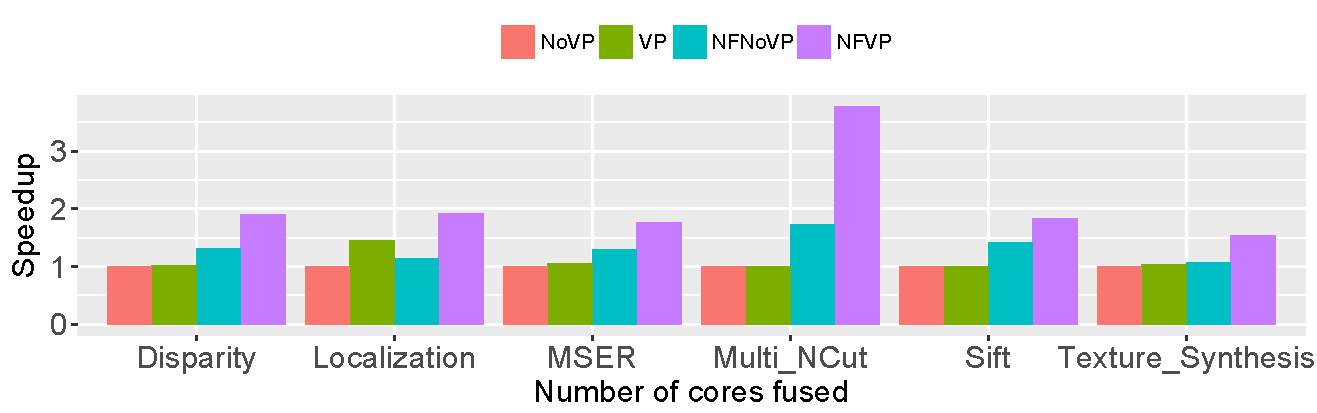
\includegraphics[width=1\textwidth]{chapter3/graphics/tempres.pdf}
    \caption{Comparing the performance of the standard fetching scheme to the new fetching scheme, with and without perfect value prediction. Higher is better}
    \label{fig:perf_pred}
\end{figure}
All configurations use perfect branch prediction as to ensure that core composition is always on the correct execution path.

Figure~\ref{fig:perf_pred} shows the speedup obtained on the SD-VBS benchmarks using the different configurations.
The baseline for this section is normal fetching scheme with no value prediction (\novp).
It is chosen as it represents a setup similar to the previous two chapters, the only difference being the perfrect branch prediction.
The number of cores composed for each benchmark using the different configurations can be found in Table~\ref{tab:conf_cores}.
As this chapter is primarily interested in getting the fastest execution times, only the fastest core composition is shown in the results.

\begin{table}[t]
  \small
  \centering
 \begin{tabular} {| l | l | l | l | l | l | }
 \hline
    & \cellcolor[gray]{0.7}Disparity & \cellcolor[gray]{0.7} Localization& \cellcolor[gray]{0.7} MSER& \cellcolor[gray]{0.7} Multi\_NCut& \cellcolor[gray]{0.7} Sift\\ \hline
 \novp   & 16  & 16 & 4  & 16& 16\\ \hline
 \vp   & 16  & 16 & 4  & 16& 16\\ \hline
 \nfnovp   & 16  & 16 & 4  & 16& 16\\ \hline
 \nfvp   & 16  & 16 & 4  & 16& 16\\ \hline
	  & \cellcolor[gray]{0.7} Stitch & \cellcolor[gray]{0.7} SVM & \cellcolor[gray]{0.7} Text. Synth & \cellcolor[gray]{0.7} Tracking&\\ \hline
\novp	 & 16& 16& 16& 16 &\\ \hline
   \vp & 16  & 16 & 4  & 16 & \\ \hline
 \nfnovp  & 16  & 16 & 4  & 16 & \\ \hline
 \nfvp   & 16  & 16 & 4  & 16 &\\ \hline

	\end{tabular}
  \caption{Number of cores composed given a configuration.}\label{tab:conf_cores}
  \vspace{1em}
\end{table}

First, it is clear that using the new fetching scheme with value prediction (\nfvp) always results in the best speedup compared to the baseline.
For \bm{Multi\_NCut}, performance is improved by almost 4x when using \nfvp.
This is a significant speedup, as Chapter~\ref{chp:cases} showed that \bm{Multi\_Ncut} was a difficult benchmark for core composition.
On average, \nfvp{} outperforms the baseline by a factor of 2x.

The results in Figure~\ref{fig:perf_pred} show that when the new fetching scheme is not paired with value prediction, the performance improvements are less important.
For example, \bm{Localization} only has a 1.10x speedup when using the \nfnovp{} configuration, compared to the 1.90x of \nfvp{}.
This is due to the fact that whilst blocks are fetched faster, the register dependencies between blocks limit the performance of core composition.
The performance limitations are caused by blocks that are further down the speculative that must wait for older blocks to write to the register file.
In fact, \vp{} outperforms \nfnovp{} on \bm{Localization}, which shows that register dependencies between blocks can make the new fetching scheme less performant than the currently implemented.

On the other hand, \bm{Multi\_NCut} with \textbf{\textit{NFNoVP}} has a 1.60x speedup compared to the baseline.
This is because \bm{Multi\_NCut} has small blocks, on average less than 10 instructions long as seen in Chapter~\ref{chp:cases} Section~\ref{sec:expl}.
When blocks are uniformly small, value prediction will not help when using the normal fetching scheme, as the composition will never be full, thus explaining why \vp{} does not perform better than the baseline.

The performance of \vp{} compared to \novp{} can be surprising as the perfect value prediction does not appear to speed up execution.
Value prediction is most useful when multiple data-dependent blocks are in flight as the data can be speculated.
However, as seen in Section~\ref{chp3:sec:fetch} the normal fetching scheme is too slow to ensure that all cores in a composition are executing blocks.
Therefore, value prediction does not benefit baseline setup, as the large core compositions are never full.

\begin{figure}[t]
    \centering
    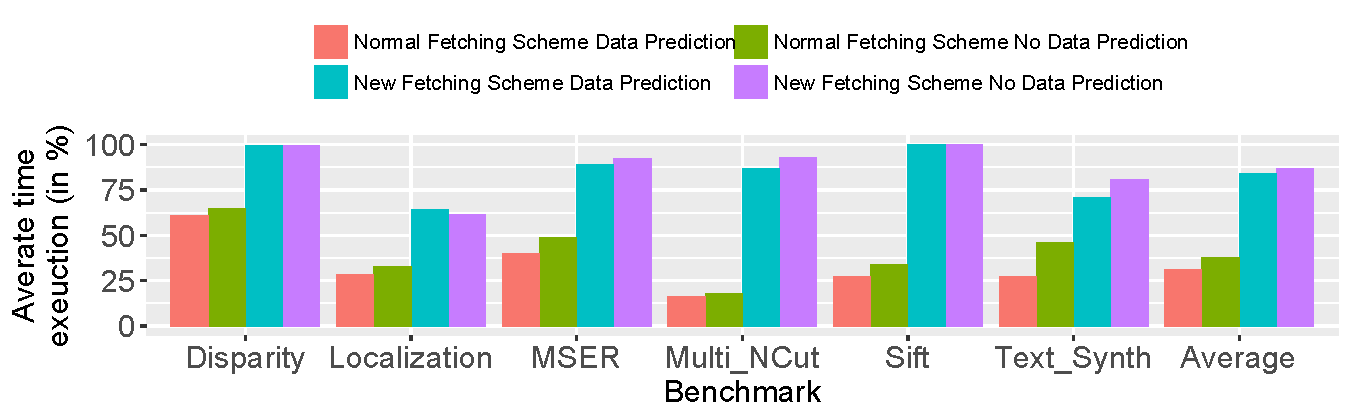
\includegraphics[width=1\textwidth]{chapter3/graphics/perf_av_cycle_exec.pdf}
    \caption{Average time each core is executing blocks (in \%) for each benchmark, using the different configurations. Higher is better.}
    \label{fig:perf_av_cycle}
	\vspace{1em}
\end{figure}

To better highlight how the normal fetching scheme hinders performance even with value prediction, the percentage of time a core in a composition was actively executing code, for each benchmark, is shown in Figure~\ref{fig:perf_av_cycle}.
For each configuration, the number of cycles each core in a composition executed instructions is averaged out and then compared to the total execution time of the application.
When the average active time of a core is close to the total execution time, this means that the composition was efficiently used, as each core executed the same amount of code.

As Figure~\ref{fig:perf_av_cycle} shows, \novp{} and \vp{} often have low active time percentages.
This is due to the fact that the current serialised block fetching scheme is slow, and thus, some cores will be innactive, waiting to receive a fetch request from another core.
The lower the percentage is, the less likely there are going to be multiple blocks on different cores in flight which in turn means value prediction is less useful.
The reason \novp{} has a higher average time of execution than \vp{} is due to the fact that in cases where value prediction is in fact usefull, it reduces the execution time of blocks.
If block execution time is reduced, this decreases the opportunity for efficient use of large core compositions due to how the fetching mechanism is slow (recall Figure~\ref{fig:new_fetch_ex} in Section~\ref{chp3:sec:fetch}).
Since value prediction is aimed at increasing instruction level parallelism (ILP)~\cite{peraisBeBop2015} it is important that cores may fetch blocks quickly in a composition.
The lack of performance differences between \novp{} and \vp{} is proof that a faster fetching scheme is required to allow core composition to benefit from value prediction.

Overall, \nfnovp{} and \nfvp{} increase the average time each core is executing code by a factor of 3x.



\subsection{Using perfect branch prediction and Block VTAGE value predictor}
\begin{figure}[t]
    \centering
    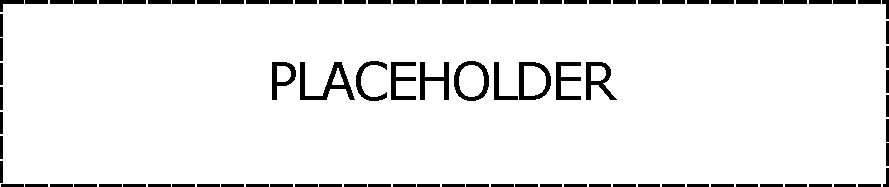
\includegraphics[width=1\textwidth]{chapter3/graphics/wip.pdf}
    \caption{Comparing the performance of the new fetching scheme, with perfect value prediction and with the VTAGE predictor. Higher is better}
    \label{fig:perf_pred}
	\vspace{1em}
\end{figure}

\subsection{Bottleneck analysis}